%% bare_jrnl.tex
%% V1.4b
%% 2015/08/26
%% by Michael Shell
%% see http://www.michaelshell.org/
%% for current contact information.
%%
%% This is a skeleton file demonstrating the use of IEEEtran.cls
%% (requires IEEEtran.cls version 1.8b or later) with an IEEE
%% journal paper.
%%
%% Support sites:
%% http://www.michaelshell.org/tex/ieeetran/
%% http://www.ctan.org/pkg/ieeetran
%% and
%% http://www.ieee.org/

%%*************************************************************************
%% Legal Notice:
%% This code is offered as-is without any warranty either expressed or
%% implied; without even the implied warranty of MERCHANTABILITY or
%% FITNESS FOR A PARTICULAR PURPOSE! 
%% User assumes all risk.
%% In no event shall the IEEE or any contributor to this code be liable for
%% any damages or losses, including, but not limited to, incidental,
%% consequential, or any other damages, resulting from the use or misuse
%% of any information contained here.
%%
%% All comments are the opinions of their respective authors and are not
%% necessarily endorsed by the IEEE.
%%
%% This work is distributed under the LaTeX Project Public License (LPPL)
%% ( http://www.latex-project.org/ ) version 1.3, and may be freely used,
%% distributed and modified. A copy of the LPPL, version 1.3, is included
%% in the base LaTeX documentation of all distributions of LaTeX released
%% 2003/12/01 or later.
%% Retain all contribution notices and credits.
%% ** Modified files should be clearly indicated as such, including  **
%% ** renaming them and changing author support contact information. **
%%*************************************************************************

\documentclass[journal]{IEEEtran}
\usepackage{pgfplots}

\ifCLASSINFOpdf
  %\usepackage[pdftex]{graphicx}
  % declare the path(s) where your graphic files are
  %\graphicspath{{img/}}
  % and their extensions so you won't have to specify these with
  % every instance of \includegraphics
  %\DeclareGraphicsExtensions{.jpg,.pdf,.jpeg,.png}
\else
  % or other class option (dvipsone, dvipdf, if not using dvips). graphicx
  % will default to the driver specified in the system graphics.cfg if no
  % driver is specified.
  % \usepackage[dvips]{graphicx}
  % declare the path(s) where your graphic files are
  % \graphicspath{{../eps/}}
  % and their extensions so you won't have to specify these with
  % every instance of \includegraphics
  % \DeclareGraphicsExtensions{.eps}
\fi
\hyphenation{op-tical net-works semi-conduc-tor}


\usepackage{soul, color}
\usepackage{listings}
\usepackage{xcolor}

\lstset { %
    language=C++,
    backgroundcolor=\color{black!5}, % set backgroundcolor
    basicstyle=\footnotesize,% basic font setting
}

\begin{document}
\title{Implementation of a Non-Blocking\\ Hashtable using C++11}
\author{Timothy~Flowers,
        Austin~Lasher,
        and~Joseph~Maag% <-this % stops a space
}

\markboth{UCF COP4520 -- Parallel Processing, Assignment 2}
{Shell \MakeLowercase{\textit{et al.}}: Bare Demo of IEEEtran.cls for IEEE Journals}
\maketitle

\begin{abstract}
In the paper “Non-blocking Hashtables with Open Addressing”, Chris Purcell and Tim Harris propose a non-blocking hashtable that utilizes buckets, probe bounds, and open addressing for standard hashtable functionality and achieves non-blocking behavior with the use of atomic lock-free operations, custom word types, and additional states. We implemented the proposed hastable model as a C++11 class utilizing C++11 features and libraries. We maintained lock-freedom with the use of the C++11 atomic library to implement hastable operations that can be performed concurrently. Our implementation was tested over a series of trials and resulted in slower performance compared to our sequential implementation. 
\end{abstract}

\section{Introduction}
\IEEEPARstart{I}{n} this paper we will describe a  sequential version of a non-blocking hashtable described by Chris Purcell and Tim Harris in their paper “Non-blocking Hashtables with Open Addressing”. We implemented the data structure a a C++11 class and performed a series of tests to assess its performance.
We will first in Section 1 describe the hashtable proposed in the original paper. Section 2 will describe the details of our C++11 implementation. Lastly, we will describe our performance tests and analyze the results to give an overall view of the efficiency of the concurrent version of the described hashtable and compare our results to our previous sequential version.


 
\section{Algorithm Description}

The non-blocking implementation of our hashtable contains three operations: Insert, Delete, and Contains. The function of these operations is described below, as well as a description of the necessary changes for a Non-Blocking implementation.

	The non-blocking hashtable utilizes open addressing to resolve conflicts. Each bucket has a bound number that is used as an upper bound on how many buckets that need to be searched during a probing sequence when looking for a key to remove, add, or find. The hashtable described implements this in a non-blocking fashion so any number of threads can be inserting or deleting with progress and accuracy guaranteed.
Keeping the bound values correct can be difficult in a concurrent environment. A thread that adds or removes a value attempts to raise or lower the bounds value at the hashed index collision position. At any time during this process, the thread can be paused by the scheduler while another 2nd thread could also add or remove a value. If that 2nd thread finishes, and the original thread resumes, the bound value it sets could now be incorrect. 

	To alleviate this, a scanning bit is packed into the word that represents the bound value. The bit and bound value can then be accessed atomically with a compare-and-swap operation in one atomic instruction. When a thread lowers a bound value, it sets the scanning bit value to 'true' when it begins scanning bound positions. When finished lowering the bounds, it checks if the scanning bit is still true at the hashed index position. If not, that means that the scanning phase was disrupted, so the process is repeated. This allows bounds to be changed atomically with the correct and accurate value.
	
	When used in parallel, keys could be duplicated as a result of concurrent insertions and deletions. The described hashtable avoids this by assigning a state to each bound position. An ‘empty’ and ‘member’ flag can be used to declare that a bucket is empty or occupied, and a bucket that is in the insertion process can be in an ‘inserting’ state. Before the insertion process and while raising its bound,it is set to a ‘visible’ state to specify it is not yet in the process of inserting. During its probing sequence for the key, it checks the states of the other buckets. If it finds an already inserted member of the same value, it can stop inserting and set it to a ‘colliding’ state. If it finds another bucket in an inserting state, it can change that bucket's state to a ‘busy’ state, signalling it to stall temporarily. Setting a state is done with a swap atomic operation so it won't conflict if another thread changes the state.
	
	To allow lock-freedom and to prevent threads from obstructing each other, a version count value is stored at each bucket to keep track of possible alterations during an insertion process. This value is stored in the same word as the state, allowing for for an atomic single instruction to obtain and set the values which allows threads to safely assist each other concurrently.

\subsection{Insert}
Insertion begins with the hashed version of the key to be inserted. The buckets are searched with an increasing number of probing jumps to find an empty bucket (or it will find that the hashtable is full, in which case it returns false). Once an empty bucket is found with a particular number of probe jumps, the bucket state at that position is set to a ‘visible’ state, and the bound is raised if necessary. The state is then set to an ‘inserting’ state. It then traverses the probing sequence to assist any other buckets that may be in an inserting process. If any buckets (or threads) are found to be inserting the same value, the original thread's bucket is set to a ‘collided’ state, and it aborts the insertion by lowering the bound and setting itself to ‘empty’.


\subsection{Remove}


\subsection{Contains}



\section{Implementation}

Our C++11 implementation of the lock-free hashtable data structure accurately models the structure described by Chris Purcell and Tim Harris by utilizing C++11 features and libraries, including its atomic library.

\subsection{C++11}
The hashtable structure is encapsulated in a C++ class called NBHashTable with a standard C++ class source file NBHashTable.cpp and header file NBHashTable.h. It uses two additional classes, ProbeBound and VersionState, which have their own respective source and header files. C++11 was chosen as our implementation language so we could utilize the thread and atomic library that is part of the C++11 standard library. NBHashTable utilizes std::atomic\_int types and compare-and-swap functions (compare\_exchange\_strong) from the atomic library for atomic access to the hashtable bucket information (bucket bound, scanning state, state, and version) for guaranteed thread safety and implementation of lock-free algorithms. std::thread objects are used in our main test classes to spawn threads and have them interact with a NBHashTable object.

\subsection{Custom Internal Data Types}
As discussed earlier, every bucket position needs several pieces of data: the key value at that bucket, the bound value, the scanning bit value, the version value, and the bucket state value. As previously mentioned, the version and state are packed within one word. In our case this was an std:: atomic\_int value. However for organizational purposes, we subclassed std:: atomic\_int into a VersionState class which has convenient static methods to extract the version number (an int) and scanning bit state (a bool) from an int word. An enum for all 6 states (busy, member, inserting, empty, collided, visible) is provided in the VersionState header file to map directly to integers. Because these two values are still packed into one atomic word, setting and loading the values is still atomic and compare-and-swap operations on a VersionState value is lock-free.
 A bucket value is represented as a C++ struct BucketT which contains a pointer to a VersionState and a key variable of type NBType, which is simply a typedef int. All buckets are in a BucketT array from which every bucket’s respective struct data can be accessed. Initially, all BucketT objects are set to a VersionState object with a version 0 and a state of VersionState::State::EMPTY, and a key value of the preprocessor macro ’EMPTY FLAG’ defined in the NBHashTable header file. In our implementation it is set to -1 to represent an empty bucket.
 
As discussed earlier, the probe value and the bound value are packed into one word. Similar to VersionState, it has been abstracted into a class, for organization, called ProbeBound which is an std::atomic\_int subclass that has convenient static functions for extracting and creating new ProbeBounds from a scanning bit value (a bool) and a bound value (an int). Just like in VersionState, atomic and lock-free functions can still be performed on a ProbeBound like any other atomic integer value.
Each bucket has a ProbeBound to hold its bound value and scanning status, and the ProbeBounds for all buckets are kept in a ProbeBound array in NBHashTable. ProbeBound values are initialized to 0.

To abstract values from VersionState and ProbeBound atomic\_int words, each class has a set of methods that take an integer word as an input, and output the needed values by performing bitwise operations to extract them. For example, to find whether the scanning bit is set in a ProbeBound (called ‘pb’ for example), you can use the ProbeBound’s int value with the atomic load() function and then call the respective ProbeBound static function: ProbeBound::isScanning(pb.load()), which will return a bool representing whether the bucket bound is in scanning mode or not. VersionState provides similar static functions to get the version value and state value. Both classes also provide constructors to make new atomic integer words with given values (such as a version integer and a state VersionState::State enum value to make a new VersionState which contains an integer packed with both values).

\subsection{Methods}
NBHashTable has three public methods that are used primarily to interact with it: remove, insert, and contains. All have a single argument of NBType, which is is defined in the header file as a typedef integer type. All arguments are expected to be greater than or equal to 0.

The implementation for these three methods all start with hashing the input value to make an associated index that is within the range of this buckets and bounds array. This hash function is simply ’(value % kSize)’ where kSize is the hashtable size.
These methods interact with the BucketT array and ProbeBound array to interact with the hashtable values. To maintain lock freedom and atomicity, a compare-and-swap function commonly used throughout these public methods (as well as private methods) to change the value of a VersionState or a ProbeBound after verifying its value. Usually this is done to make sure no other thread has changed a value in the middle of the process, such as in the public ‘insert’ method and the private ‘conditionallyLowerBound’ method. For this we use the compare\_exchange\_strong method from the atomic C++11 library to perform look-free compare and swaps of ProbeBounds and VersionStates.

There are several private methods to help perform NBHashTable operations. ‘conditionallyLowerBound’ is a probing process used to lower the bound at a particular bucket value. It performs the probing process and atomically uses the scanning value in each bucket’s VersionState it encounters for lock-free interaction. ‘conditionallyRaiseBound’ raises a bucket’s bound, which is used when inserting a value. It uses the lock-free ‘compare\_exchange\_strong’ to make sure the new ProbeBound value is set, and that the original value is the same as it was at the beginning at the process. If it has changed, it repeats the probing process to find its new bound value.

ProbeBound and VersionState values are read atomically and without locking. The values stored in their respective int word are extracted with public static methods within each of their respective classes, such as VersionString::getVersion() and ProbeBound::getBound() (both of which take an integer argument).

\subsection{Lock-Freedom}

\section{Testing and Performance}

To compare our algorithm to the original description, we set up several testing suites that implemented our NBHashTable class. In the previous assignment, we focused on both correctness, and execution time. This time around, as we have added some additional structures to support non-sequential loads, we required several new tests in addition to the previous tests.

The first new test is our Atomic Types test file, "atomictypes.cpp". This program allowed us to create test cases for our ProbeBound and VersionState classes. As the paper showed, we used a bit-stealing technique to combine the probe bound and scanning bit into a single memory word, so a single compare-and-swap operation could update this value. The same process needed to be done for the Version and bucket state variables, except the bucket state required three bits as there were six possible states.

The second new test file is titled "instructions.cpp", and allows us to input exact numbers we wanted inserted and deleted. This way, we can set up even more specific tests and make sure that each function was working appropriately.


\subsection{Correctness}

Correctness is difficult to measure for all cases. Unlike execution time, it would be difficult to create a testing suite to measure correctness that randomly generates numbers. It would randomly have to generate insertions and deletions of numbers, and from that compare it to a "correct" output, that it would also have to generate. How can we be sure that the output it created was actually correct for every case? There is no way to be sure, as there could be a fault in our procedure that generates a "correct" output. A false positive, in this case, would be likely.

Our approach to measuring the correctness of the algorithm, instead, was to create several test cases. The idea is that we can create test cases, and compare the actual result to an expected result we retrieved on paper. With this method, we can create many different tricky test cases, and see how they perform individually. From each tricky test case, we were thereby able to refine our implementation to be certain of its correctness, and kept refining different portions of code until we were certain it was correct.

We've added a new file to verify correctness on this submission as mentioned earlier, "instructions.cpp". The goal of this new program is to read in from standard input (or a piped file) the number of threads to create, the size of our table, and a list of instructions to perform. The instructions are specific insertions, deletions, and contains operations. The program will read this file, follow it as said, and print results as it inserts them into the hash table. This way, we can create inputs with even trickier general test cases and visually see how the insertions and deletions are affecting the table.

To run our correctness file, we've added a GNU make target called "instructions" to our Makefile. The built executable will be placed inside the build/ directory. Once built, input can be given to the executable through file piping. We've provided an example file, "instructions.in" and a description of the input format inside the source code file.

Our other two correctness files are 'correctness1.cpp' and 'correctness2.cpp', which are left over from our last project for comparison. These two older files can be built using our GNU Makefile with the target "make correctness". This will make two corresponding executables, correctness1 and correctness2 under the build/ directory. These can be run to show our testing methodology, and the proof of our algorithm can be visually seen.



\subsection{Execution time}

Execution time is important to test because it allows us to compare the specific operations of the algorithm and determine how it should be used most efficiently. It also allows us to compare our implementation to the expected time from the original paper, and potentially see the limits of our currently sequential solution.

Our goal is to measure execution for a potentially random set of data in bulk, and measure the approximate execution time depending on the number of threads. We also hope to visually see a correlation between the number of operations performed and the resulting execution time for those set of operations. To do this, we created a C++ program (executiontime.cpp) that we can run multiple times with different parameters, and will show the average execution time on the given parameters.

With this goal in mind, we approached the program by spawning some number of threads, and performed 500,000 operations on each of those threads. These were either insert() operations, delete() operations, or contains() operations. The distribution of each of these was modified into six different cases, shown in Table 1 below.

\begin{table}[h]
\centering
\begin{center}
\begin{tabular}{ |c|c|c|c| } 
 \hline
 Trial \# & insert() & delete() & contains() \\ 
 \hline
 1 & 75\% & 25\% & 0\% \\ 
 2 & 25\% & 75\% & 0\% \\ 
 3 & 50\% & 50\% & 0\% \\ 
 4 & 45\% & 10\% & 45\% \\ 
 5 & 10\% & 45\% & 45\% \\ 
 6 & 33\% & 33\% & 34\% \\ 
 \hline
\end{tabular}
\end{center}
\caption{Distribution of operations for each trial.}
\end{table}


Our C++ program takes four command-line arguments. The first is the integer number of threads. If no arguments are specified, the default distribution is used, and the program will ask how many threads to perform on. The first argument is the number of threads. Next are three arguments: three different percent chances for our three different operations to be performed. The first corresponds to the weighted probability of an insert operation, the second a deletion, and lastly our look-up operation (contains.)

The program will automatically run each operation with a random integer between 1 and 100, and perform these operations on a hashtable with only 50 slots. These options are customizable inside the source C++ file as \#define constants.

Because we want our test results to reflect an accurate average timing for normal use, we decided to each of our tests multiple times, timing each one, and average the results together. This was done directly inside the coded file. The number of average trials is configurable as well, and the program will print out the timing for each trial. By default, we have configured this to time each trial four times, and print the average of each measurement.

Using this program, we were able to create a huge GNU Makefile that automated our tests, and piped the output to a testing directory. The very same Makefile is available in the included package, and can be run using the target "make executionTimeTests", as described in the README file.

These methods aren't any different from our previous submission, in fact they are exactly the same. We moved the exact same files over and are using the exact same make build targets. This way, we can see the exact difference in performance of our new implementation compared to the previous sequential method.

\subsection{Results}

The overall results of each of our execution time trials, this time around, cannot be shown in a single graph. To visualize a basic sense of the maximum time increase over both versions, we've included the graph below to compare this version to the sequential version. For all of the following graphs, the blue results represent our previous sequential solution, while the red represents our new non-blocking version. Our analysis of these results is included in the following section.

\begin{figure}[!t]
	\centering
	
	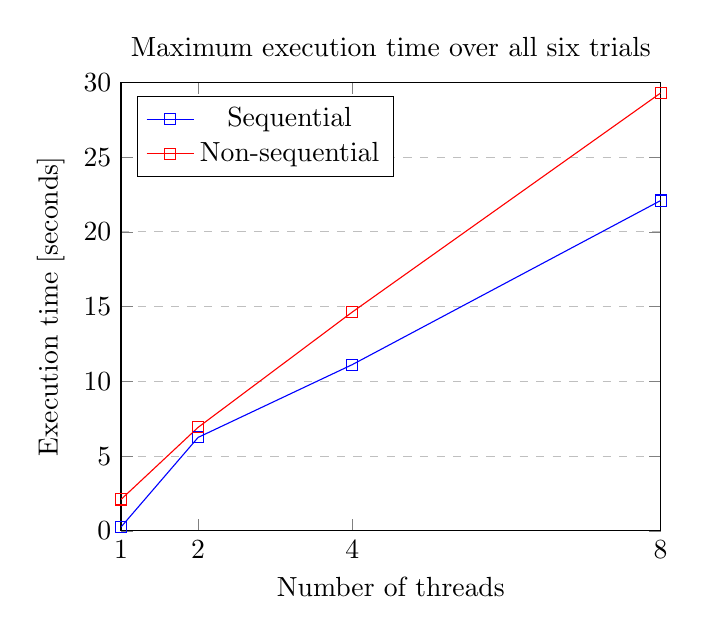
\begin{tikzpicture}
	
	\begin{axis}[
	    title={Maximum execution time over all six trials},
	    xlabel={Number of threads},
	    ylabel={Execution time [seconds]},
	    xmin=1, xmax=8,
	    ymin=0, ymax=30,
	    xtick={1,2,4,8},
	    ytick={0, 5, 10, 15, 20, 25, 30},
    	legend pos=north west,
	    ymajorgrids=true,
	    grid style=dashed,
	]
	
		
	\addplot[
	    color=blue,
	    mark=square,
	    ]
	    coordinates {
	    (1, 0.253422)(2, 6.25)(4, 11.121)(8, 22.1)
	    };
	\addplot[
	    color=red,
	    mark=square,
	    ]
	    coordinates {
	    (1, 2.1)(2, 6.922261)(4, 14.639601)(8, 29.296855)
	    };
	    
	\legend{Sequential, Non-sequential}
	
	\end{axis}
		
	\end{tikzpicture}
	%\label{Test figure}
\end{figure}


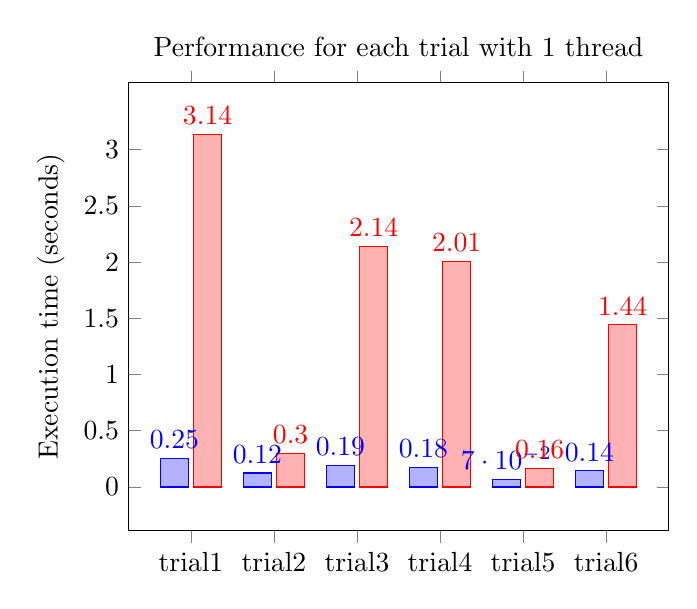
\begin{tikzpicture}
\begin{axis}[
    ybar,
    enlargelimits=0.15,
    legend style={at={(0.5,-0.15)},
      anchor=north,legend columns=-1},
    title={Performance for each trial with 1 thread},
    ylabel={Execution time (seconds)},
    symbolic x coords={trial1,trial2,trial3,trial4,trial5, trial6},
    xtick=data,
    ytick={0,0.5,1.0,1.5,2.0,2.5,3.0},
    nodes near coords,
    nodes near coords align={vertical},
    ]
\addplot coordinates {(trial1,0.253422) (trial2, 0.123798) (trial3,0.191336)(trial4,0.176446)(trial5,0.07)(trial6,0.143335)};
\addplot coordinates {(trial1,3.137997) (trial2, 0.299298) (trial3,2.140433)(trial4,2.007891)(trial5,0.163410)(trial6,1.441663)};

\end{axis}	
\end{tikzpicture}

\hfill\\

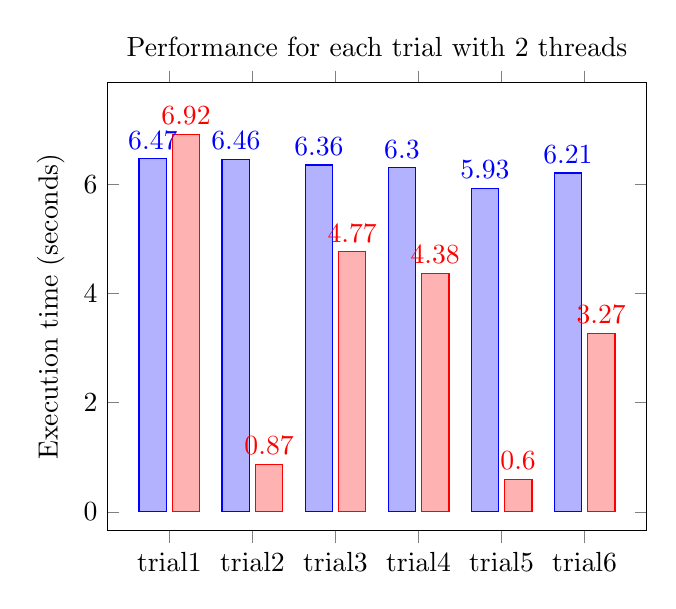
\begin{tikzpicture}
\begin{axis}[
    ybar,
    enlargelimits=0.15,
    legend style={at={(0.5,-0.15)},
      anchor=north,legend columns=-1},
    title={Performance for each trial with 2 threads},
    ylabel={Execution time (seconds)},
    symbolic x coords={trial1,trial2,trial3,trial4,trial5, trial6},
    xtick=data,
    nodes near coords,
    nodes near coords align={vertical},
    ]
\addplot coordinates {(trial1, 6.470939) (trial2, 6.456186) (trial3,6.357836)(trial4,6.304448)(trial5,5.929456)(trial6,6.211829)};
\addplot coordinates {(trial1, 6.922261) (trial2,  0.866337) (trial3, 4.767575)(trial4, 4.375773)(trial5, 0.601312)(trial6, 3.270004)};
\end{axis}	
\end{tikzpicture}

\hfill\\
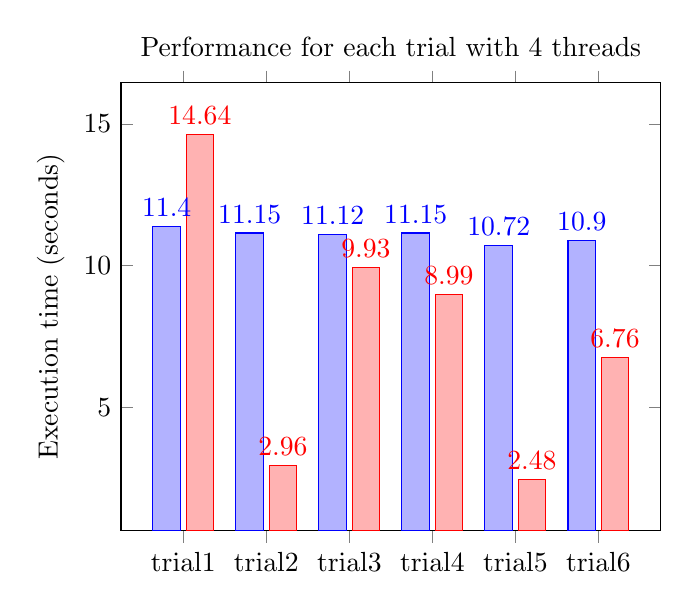
\begin{tikzpicture}
\begin{axis}[
    ybar,
    enlargelimits=0.15,
    legend style={at={(0.5,-0.15)},
      anchor=north,legend columns=-1},
    title={Performance for each trial with 4 threads},
    ylabel={Execution time (seconds)},
    symbolic x coords={trial1,trial2,trial3,trial4,trial5, trial6},
    xtick=data,
    nodes near coords,
    nodes near coords align={vertical},
    ]
\addplot coordinates {(trial1, 11.397211) (trial2,  11.154437) (trial3, 11.117342)(trial4, 11.154646)(trial5, 10.723320)(trial6, 10.902162)};
\addplot coordinates {(trial1, 14.639601) (trial2,  2.960299) (trial3, 9.934485)(trial4, 8.993448)(trial5, 2.476551)(trial6, 6.756403)};

\end{axis}	
\end{tikzpicture}

\hfill\\

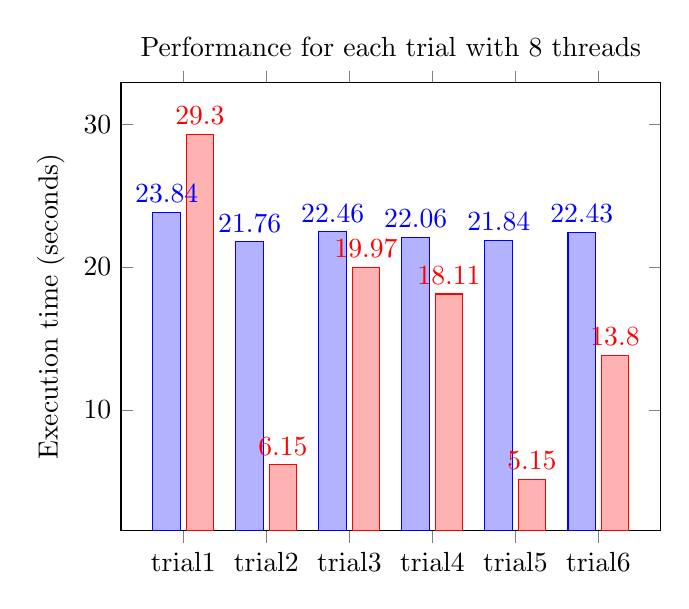
\begin{tikzpicture}
\begin{axis}[
    ybar,
    enlargelimits=0.15,
    legend style={at={(0.5,-0.15)},
      anchor=north,legend columns=-1},
    title={Performance for each trial with 8 threads},
    ylabel={Execution time (seconds)},
    symbolic x coords={trial1,trial2,trial3,trial4,trial5, trial6},
    xtick=data,
    nodes near coords,
    nodes near coords align={vertical},
    ]
\addplot coordinates {(trial1, 23.836776) (trial2,  21.758258) (trial3, 22.457724)(trial4, 22.058291)(trial5, 21.841913)(trial6, 22.432596)};
\addplot coordinates {(trial1, 29.296855) (trial2,  6.150445) (trial3, 19.973269)(trial4, 18.112122)(trial5, 5.153033)(trial6, 13.796656)};
\end{axis}	
\end{tikzpicture}

\hfill\\

\section{Execution Time Analysis}

We originally speculated that a non-blocking version of this code would considerably decrease our load, and what we found was much more interesting. 

For a single thread, we can clearly see that the execution time was much larger. We think this makes sense, as we've added a lot of overhead to our new code that the old code didn't have to go through for an insertion. It appears as though trials 2 and 5 for the single threaded results were comparable to the previous results, and we feel that's because of the low number of insertion operations. That must mean for a single thread, insertions take significantly longer. That makes sense, as the work load cannot be distributed at all, and the new features have added a lot of overhead on adding an element that's reduced as the load becomes more distributed amongst more threads.

The second interesting fact is that trial 1 takes significantly longer amongst all graphs. When looking at the distribution, it's clear to see that trial 1 performs a significantly high number of insertions. It's clear that this new algorithm has added some extra contention among the insertion operations.

We can see that generally, with the exception of trial 1, as the number of threads decrease, the execution time marginally decreases as well. On all tests, trials two and five were significantly faster than the old version for all but the 1-threaded test, that's because our structure can perform contains and deletion operations much faster than an insertion. Now that the structure doesn't have to wait for a lock to release, it's free to perform those much faster than before.

Otherwise, the results were surprisingly comparable than the previous method. When reading the paper, we were convinced we were working with black magic. That no matter what, a method this interesting had to deliver breathtakingly fast results. Though these improvements are definitely seen on trials 2 and 5 for results with multiple threads, we admit the results are not as startling as we originally thought.


\section{Conclusion}

The non-blocking hashtable proposed by Chris Purcell and Tim Harris uses a number of atomic operations, lock-free operations, and specialized data types to achieve non-blocking functionality.  Our implementation followed the provided algorithms precisely with slight modifications for the use of C++11. 


\ifCLASSOPTIONcaptionsoff
  \newpage
\fi



\begin{thebibliography}{1}

\bibitem{IEEEhowto:kopka}

C.~Purcell and T.~Harris, \emph{Non-blocking Hashtables with Open Addressing}.\hskip 1em plus
  0.5em minus 0.4em\relax Springer-Verlag, Berlin, Heidelberg, 2005.

\end{thebibliography}

\end{document}

